% !TeX program = xelatex
% Chọn main.tex làm Main document; biên dịch bằng XeLaTeX.
\documentclass[conference,a4paper]{IEEEtran}
\usepackage{fontspec}
\IfFontExistsTF{TeX Gyre Termes}
  {\setmainfont{TeX Gyre Termes}}
  {\setmainfont{Liberation Serif}}
\IfFontExistsTF{TeX Gyre Heros}
  {\setsansfont{TeX Gyre Heros}}
  {\setsansfont{Liberation Sans}}
\IfFontExistsTF{DejaVu Sans Mono}
  {\setmonofont{DejaVu Sans Mono}[Scale=MatchLowercase]}
  {\setmonofont{Latin Modern Mono}[Scale=MatchLowercase]}
\usepackage{cite}
\usepackage{amsmath,amssymb,amsfonts}
\usepackage{graphicx}
\usepackage{booktabs,tabularx,array}
\usepackage{listings}
\usepackage{xcolor}
\usepackage{balance}
\usepackage[hidelinks,unicode]{hyperref}
\urlstyle{same}
\renewcommand{\abstractname}{Tóm tắt}
\renewcommand{\IEEEkeywordsname}{Từ khóa}
\renewcommand{\refname}{Tài liệu tham khảo}
\renewcommand{\figurename}{Hình}
\renewcommand{\tablename}{Bảng}
\newcolumntype{Y}{>{\raggedright\arraybackslash}X}
\lstset{basicstyle=\ttfamily\scriptsize,breaklines=true,
  columns=fullflexible,keepspaces=true,showstringspaces=false,
  frame=single,rulecolor=\color{black!25},captionpos=b,
  aboveskip=6pt,belowskip=6pt}
\newcommand{\code}[1]{\texttt{#1}}

\begin{document}
\title{Báo cáo cuối kỳ: Nhập môn Trí tuệ nhân tạo}
% Điền thành viên theo nhóm thực tế; không dùng tên có sẵn trong mẫu.
\author{\IEEEauthorblockN{Họ tên / MSSV: \underline{\hspace{3cm}}}
\IEEEauthorblockA{Lớp / Nhóm: \underline{\hspace{3cm}}\\
Trường / Khoa: \underline{\hspace{3cm}}\\
Giảng viên: \underline{\hspace{3cm}}}}
\maketitle

% Bổ sung tóm tắt Bài 1 và Bài 3 khi hai thành viên hoàn thiện nội dung.
\begin{abstract}
Phần tìm kiếm đối kháng mô hình hóa Tank Battle thành trò chơi hai bên
tổng bằng không và triển khai bốn cấu hình: Minimax, Alpha-Beta,
Heuristic Minimax và Heuristic Minimax kết hợp Alpha-Beta. Chương trình
dùng Python/Pygame, tổ chức hướng đối tượng, có giao diện quan sát
quyết định và cơ chế nạp agent bên ngoài. Thực nghiệm gồm 240 lượt tìm
kiếm trên cùng trạng thái và 60 trận đổi bên. Các cặp cùng hàm đánh giá
khớp giá trị; Alpha-Beta giảm số nút trên bộ thử. Heuristic cung cấp
tín hiệu chiến thuật ở lá chưa kết thúc với chi phí đánh giá bổ sung.
Kết quả được giới hạn trong các bản đồ, độ sâu và môi trường đã đo.
\end{abstract}
\begin{IEEEkeywords}
trí tuệ nhân tạo, tìm kiếm đối kháng, Minimax, Alpha-Beta, heuristic,
Tank Battle, Pygame.
\end{IEEEkeywords}

% Ba file tương ứng ba bài toán; chỉ task2.tex đã được viết đầy đủ.
% File nội dung Bài toán 1. Không thêm documentclass/begin{document}.
% Thay tên và bổ sung nội dung theo đề thực tế; chưa có thông tin để viết thay.
\section{Bài toán 1: Tên bài toán cần bổ sung}
\label{sec:task1}
\textit{Phần nội dung Bài toán 1 do thành viên phụ trách bổ sung.}
% \subsection{Phát biểu và mô hình hóa bài toán}
% \subsection{Thuật toán và cài đặt}
% \subsection{Thực nghiệm và phân tích kết quả}
% \subsection{Kết luận và hạn chế}

% Phần Bài toán 2: nội dung độc lập, ghép qua input trong main.tex.
% Nhãn t2:* tránh trùng với hai bài còn lại.
\section{Bài toán 2: Adversarial Search --- Tank Battle}
\label{sec:task2}

\subsection{Mục tiêu và phạm vi}
Đề bài yêu cầu công thức hóa game tank thành trò chơi tổng bằng không,
triển khai và so sánh bốn cấu hình tìm kiếm đối kháng trong cùng điều
kiện, xây dựng giao diện Pygame và cơ chế nhập thuật toán của nhóm khác
\cite{assignment}. Hai bên cần bảo vệ tank/căn cứ của mình và phá hủy
tank hoặc căn cứ đối thủ. Việc chọn hành động phải xét phản ứng của
đối phương, thay vì chỉ đi theo một đường có sẵn.

Chương trình phát triển từ mã nguồn/tài nguyên Battle City
\cite{battlecity}; luật, mô hình tìm kiếm và thí nghiệm được triển khai
cho yêu cầu của đề \cite{project}. Phân tích tập trung vào chế độ hai
AI, \emph{AI WARGAME}. Chế độ người chơi đấu bốn NPC, \emph{SOLO SORTIE},
là phần mở rộng: mỗi NPC lập kế hoạch trên bản chiếu hai xe, không phải
cây đối kháng đầy đủ năm tác nhân. Số liệu dưới đây chỉ dùng bài toán
hai bên.

\subsection{Công thức hóa trò chơi tổng bằng không}
\subsubsection{Người chơi và trạng thái}
Hai bên có chỉ số $p\in\{0,1\}$, luân phiên hành động. Tại mỗi lần tìm
kiếm, bên cần chọn nước là MAX, bên còn lại là MIN; MAX không cố định
là P0. Môi trường xác định và quan sát đầy đủ: cùng trạng thái, cùng
hành động sinh cùng trạng thái kế tiếp.

Trạng thái được mô tả bởi
\begin{equation}
s=(M,T_0,T_1,B_0,B_1,L,p,c),
\label{t2:eq:state}
\end{equation}
trong đó $M$ chứa kích thước lưới, thép và HP từng ô gạch;
$T_i=(r_i,c_i,d_i,h_i)$ chứa vị trí, hướng và HP tank; $B_i$ chứa vị trí
và HP căn cứ; $L$ là tập đạn với vị trí, hướng, chủ sở hữu; $p$ là bên
tới lượt và $c$ là cycle phục vụ điều phối/hiển thị. Cycle không tự
tạo trạng thái kết thúc.

\subsubsection{Hành động hợp lệ và hàm chuyển}
Một tank có sáu loại hành động:
\begin{equation}
\begin{split}
A=\{&\code{MOVE\_UP},\code{MOVE\_DOWN},\code{MOVE\_LEFT},\\
&\code{MOVE\_RIGHT},\code{FIRE},\code{STAY}\}.
\end{split}
\end{equation}
Tập $A(s)$ được tạo bởi \code{legal\_actions}. Khi game chưa kết thúc,
FIRE và STAY hợp lệ. Một MOVE hợp lệ nếu ô phía đó trống hoặc hướng
được chọn khác hướng hiện tại. Ô trống cho phép quay và đi một ô; ô
bị chặn cho phép chỉ quay tại chỗ. MOVE vào ô bị chặn theo đúng hướng
đang nhìn được bỏ vì tương đương STAY. Tank không đi qua thép, gạch,
tank khác, căn cứ hoặc biên lưới. Đạn không chặn di chuyển nhưng có
thể gây sát thương khi tank bước vào ô chứa đạn.

Hàm $T(s,a)$ sao chép trạng thái rồi áp dụng hành động $a$. FIRE sinh
một viên đạn theo hướng hiện tại; STAY bỏ lượt. Một cycle được mô hình
hóa theo thứ tự P0 hành động, P1 hành động, sau đó đạn tiến tối đa ba ô.
Va chạm được kiểm tra sau từng bước một ô; viên đạn dừng tại thực thể
đầu tiên trúng phải, không xuyên tiếp sau khi gây sát thương. Đạn ra
ngoài lưới bị loại. Bảng~\ref{t2:tab:hp} thể hiện HP/sát thương theo đề.

\begin{table}[t]
\caption{HP khởi tạo và sát thương theo yêu cầu đề}
\label{t2:tab:hp}
\centering
\begin{tabular}{lrr}
\toprule
Thực thể & HP khởi tạo & Sát thương mỗi hit\\
\midrule
Tank & 6 & 1\\
Căn cứ & 9 & 1\\
Tường gạch & 3 & 1\\
\bottomrule
\end{tabular}
\end{table}

\subsubsection{Terminal và utility}
Bên $i$ thua nếu tank hoặc căn cứ của bên đó hết HP. Do đó
\begin{equation}
\operatorname{Terminal}(s)\iff
\exists i:\ h(T_i)\leq0\ \lor\ h(B_i)\leq0.
\end{equation}
Nếu chỉ một bên thua thì bên còn lại thắng. Nếu cả hai bên đồng thời
thỏa điều kiện thua trong cùng cập nhật thì quy ước hòa. Tank và base
của cùng một bên bị phá không tạo hòa: bên đó vẫn thua nếu đối phương
còn sống. Utility theo góc nhìn $p$ là
\begin{equation}
U_p(s)=\begin{cases}
+10000,&p\text{ thắng},\\
-10000,&p\text{ thua},\\
0,&\text{hai bên cùng bị phá}.
\end{cases}
\end{equation}
Vì $U_0(s)=-U_1(s)$ nên tổng utility bằng không. Trong search, tại nút
terminal còn $d$ ply, điểm thắng được cộng $d$, điểm thua bị trừ $d$,
điểm hòa giữ 0; nhờ đó ưu tiên thắng sớm và trì hoãn thua. Quy tắc này
áp dụng giống nhau cho cả bốn cấu hình.

\subsubsection{Các giả định ngoài mô tả chi tiết của đề}
Các quy ước sau được dùng nhất quán trong mô phỏng và chơi thật:
\begin{itemize}
\item P1 quan sát trạng thái sau hành động P0. Đây là mô hình luân
phiên thông tin đầy đủ, không phải chọn hành động đồng thời kín.
\item Thép không phá được. Đạn đang bay vào cùng ô hoặc hoán đổi ô
trong một bước sẽ triệt tiêu nếu chưa va chạm thực thể.
\item Tank bước vào ô có đạn mất HP bằng số viên tại ô và loại các
viên đó. Đạn có thể gây sát thương tank/base của chính phe bắn.
\item Sát thương ở cùng bước đạn được cộng trước khi xác định phá hủy;
phá hủy đồng thời hai bên được tính hòa.
\item Một depth là một \emph{ply}, tức một hành động của một bên.
Giới hạn cycle của thí nghiệm chỉ dừng bộ chạy, không thuộc luật game
hoặc utility của cây tìm kiếm.
\end{itemize}

\subsection{Bốn cấu hình tìm kiếm đối kháng}
\subsubsection{Cách đánh giá lá}
Bảng~\ref{t2:tab:modes} nêu đúng bốn cấu hình cần so sánh. Hai bản
thuần dùng \code{TerminalEvaluator}: trạng thái terminal dùng utility,
lá chưa terminal tại ngưỡng depth có giá trị 0. Hai bản heuristic chỉ
thay giá trị lá chưa terminal bằng $H(s,p)$, giữ nguyên luật và utility.

\begin{table}[t]
\caption{Bốn cấu hình chính; MM = Minimax, AB = Alpha-Beta}
\label{t2:tab:modes}
\centering\small
\begin{tabularx}{\columnwidth}{lYc}
\toprule
Cấu hình & Lá chưa terminal & Cắt tỉa\\
\midrule
MM & 0 (terminal-only) & Không\\
AB & 0 (terminal-only) & Có\\
H-MM & $H(s,p)$ & Không\\
H-AB & Cùng $H(s,p)$ & Có\\
\bottomrule
\end{tabularx}
\end{table}

Đây là các bản tìm kiếm giới hạn độ sâu; hai bản thuần không vét cạn
toàn bộ ván tới terminal. Điểm 0 ở chân trời là thiếu thông tin phân
biệt, không khẳng định ván sẽ hòa. Cả bốn cấu hình không dùng bảng
chuyển vị (TT) hoặc phạt trạng thái lặp trong phép so sánh chính.

\subsubsection{Minimax}
Gọi $m$ là bên đang được tối ưu và $E$ là evaluator của cấu hình.
Đặt $U_m^{(d)}(s)=U_m(s)+d\,\operatorname{sgn}U_m(s)$ và
$v_a=V(T(s,a),d-1;m)$. Giá trị tìm kiếm được định nghĩa bởi
\begin{equation}
V(s,d;m)=\begin{cases}
U_m^{(d)}(s),&s\text{ terminal},\\
E(s,m),&d=0,\ s\text{ chưa terminal},\\
\max\limits_{a\in A(s)}v_a,&p(s)=m,\\
\min\limits_{a\in A(s)}v_a,&p(s)\neq m.
\end{cases}
\label{t2:eq:minimax}
\end{equation}
Tại gốc, chọn hành động có giá trị lớn nhất sau khi xét phản ứng tốt
nhất của MIN. Thuật toán chỉ tối ưu theo mô hình và độ sâu đã duyệt,
không bảo đảm thắng cả ván. Với hệ số phân nhánh $b\leq6$ và độ sâu
$d$, thời gian trường hợp xấu nhất là $O(b^d)$. Duyệt sâu dùng ngăn xếp
theo độ sâu, nhưng mỗi nút vẫn cần sao chép trạng thái và UI có thể
lưu nước phục vụ giải thích.

\subsubsection{Alpha-Beta}
Alpha-Beta dùng cùng MAX/MIN và evaluator, duy trì $\alpha$ là cận
dưới từ lựa chọn của MAX và $\beta$ là cận trên từ MIN. Sau khi cập
nhật giá trị ở MAX, cập nhật $\alpha$; ở MIN, cập nhật $\beta$. Khi
$\alpha\geq\beta$, bỏ các hành động chưa xét trong nhánh vì chúng
không thể cải thiện quyết định tại tổ tiên.

Nếu hoàn tất cùng depth trên cùng trạng thái/evaluator, Alpha-Beta
giữ nguyên giá trị tối ưu của Minimax. Nhiều nước đồng điểm có thể
dẫn đến lựa chọn khác nhau; kiểm tra tính đúng cần so giá trị và việc
hành động thuộc tập tối ưu, không yêu cầu mọi nước trùng nhau. Trường
hợp xấu nhất vẫn $O(b^d)$; thứ tự duyệt lý tưởng có thể đạt gần
$O(b^{d/2})$. Cài đặt hiện tại sắp xếp con ở gốc cho cả hai thuật toán.

\subsubsection{Độ sâu và giới hạn thời gian}
UI cho chọn depth 1--8, mặc định 4; ngân sách 60/120/250 ms hoặc
FULL DEPTH. Khi có deadline, iterative deepening thử depth tăng dần,
trả kết quả vòng hoàn tất cuối cùng. Nếu chưa hoàn tất depth 1, trả
một hành động hợp lệ dự phòng. Ngân sách là mềm vì một lần đánh giá
đang chạy không bị cưỡng bức ngắt. FULL DEPTH chỉ hoàn tất độ sâu đã
chọn, không có nghĩa tìm hết toàn bộ game.

\subsubsection{Vì sao bản thuần có thể đứng bắn}
Ở depth nhỏ, nếu mọi lá chưa kết thúc đều bằng 0, nhiều hành động gốc
có thể đồng điểm. FIRE đứng đầu thứ tự ổn định nên có thể được chọn
liên tiếp. Đây là giới hạn của đánh giá lá, không phải Minimax/AB
không quyết định được di chuyển. Khi cây nhìn thấy khác biệt thắng/
thua, bản thuần vẫn chọn được nước né hoặc tấn công. Kiểm thử dùng
snapshot tank còn 1 HP, đạn sắp trúng và depth 4 cho thấy bản thuần
chọn né trái/phải; đây là trạng thái giữa ván, không thay HP khởi tạo 6
và không thay thế tập map benchmark.

\subsection{Hàm heuristic và ý nghĩa chiến thuật}
Với $e=1-p$, điểm trạng thái chưa terminal là
\begin{equation}
\begin{split}
H(s,p)={}&100\,[h(B_p)-h(B_e)]\\
&+80\,[h(T_p)-h(T_e)]\\
&+10\,(D_e-D_p)+30\,(A_p-A_e)\\
&+60\,(R_e-R_p).
\end{split}
\label{t2:eq:heuristic}
\end{equation}
$D_i$ là chi phí ước lượng tới vị trí bắn căn cứ địch; $A_i$ là chất
lượng hướng ngắm; $R_i$ là thiệt hại dự báo lên bên $i$. Khoảng cách
và nguy cơ của mình nhỏ hơn là tốt hơn, nên hai thành phần này dùng
``đối thủ trừ mình'', khác dấu với HP và ngắm.

\subsubsection{Vật chất và vị trí bắn}
Chênh lệch HP thưởng giữ tank/base của mình và gây sát thương địch.
Chi phí $D_i$ được tính bằng Dijkstra ngược trên cặp (ô, hướng), bắt
đầu từ những vị trí có thể bắn về căn cứ địch. Chi phí gồm hành động
bắn, ước lượng thời gian bay, HP gạch trên tia, di chuyển và đổi hướng
khi cần. Đường không xuyên thép hoặc đi vào ô căn cứ. Khoảng cách
không tìm được hoặc quá xa được giới hạn ở 99.

Mô hình đường đi là thư giãn tĩnh: chưa xét tank khác sẽ chuyển động
và chưa mô phỏng đầy đủ thời gian chờ đạn phá từng lớp gạch. Vì vậy
$D_i$ là tín hiệu dẫn hướng, không phải số lượt thắng được bảo đảm.
Luật chuyển trạng thái trong cây vẫn được engine tính chính xác.

\subsubsection{Ngắm và nguy cơ đạn}
$A_i$ dò tia theo hướng nòng súng. Ngắm mục tiêu địch có điểm dương,
ngắm phe mình có điểm âm, thép chặn tia không tạo lợi thế; có gạch
trước mục tiêu thì điểm giảm theo HP gạch phải phá. Mục tiêu base
được coi trọng hơn tank trong điểm ngắm trực tiếp.

$R_i$ được ước lượng bằng cách sao chép trạng thái và gọi cùng cơ
chế va chạm đạn tối đa ba cycle, giả sử các tank giữ nguyên vị trí và
không sinh đạn mới. Thiệt hại xa được chiết khấu theo cycle; base và
thực thể ít HP có trọng số nguy hiểm cao hơn. Dự báo xét tường chặn,
đạn triệt tiêu và sát thương phe mình. Đây là nguy cơ nếu giữ vị trí,
không khẳng định đối thủ không thể né.

Các thành phần lấy chênh lệch hai bên nên $H(s,p)=-H(s,e)$. Kết quả
được chặn trong $[-9900,9900]$ để utility terminal luôn trội hơn.
Trọng số chọn thủ công, chưa được tối ưu hoặc kiểm tra độ nhạy.
Cache khoảng cách có giới hạn 512 mục, khóa phụ thuộc địa hình, HP
gạch và căn cứ; đây là cache evaluator, không phải TT tìm kiếm.

\subsection{Thiết kế hướng đối tượng và giao diện Pygame}
\subsubsection{Tổ chức chương trình}
\code{GameState} trong \code{game.py} quản lý trạng thái, hành động,
va chạm và terminal. \code{SearchAlgorithm} có hai lớp dẫn xuất
\code{Minimax}, \code{AlphaBeta}. Các evaluator chia sẻ giao diện
\code{evaluate(state, me)}; \code{HeuristicEvaluator} kế thừa phần
vật chất từ \code{SimpleEvaluator}, còn hai mode thuần trực tiếp dùng
\code{TerminalEvaluator}. \code{Agent}/\code{SearchAgent} thống nhất
giao thức chọn hành động; \code{Match}/\code{AIBattle} điều phối và
hiển thị. Tách biệt này cho phép đổi thuật toán mà vẫn dùng chung
luật và UI, đáp ứng tổ chức hướng đối tượng.

Luồng xử lý là UI yêu cầu agent chọn nước trên bản sao, search gọi
chuyển trạng thái/evaluator, rồi Match kiểm tra và áp dụng hành động
vào trạng thái thật. Tìm kiếm chạy ở luồng riêng để cửa sổ tiếp tục
nhận sự kiện; không có nhiều lượt được áp dụng đồng thời. Việc thử
nước trong cây không thay đổi trạng thái đang chơi.

\subsubsection{Quan sát quyết định trên UI}
Pygame \cite{pygame} hiển thị bản đồ, HP tank/base, hành động, thời
gian, số nút và depth thực. Chế độ AI WARGAME cho hai AI tự đấu, không
chèn điều khiển bàn phím vào một bên. Phím P dừng, N thực hiện một
hành động AI, Tab mở phân tích, V bật tia ngắm, +/- đổi tốc độ trình
diễn và Esc quay lại cấu hình. Hình~\ref{t2:fig:ui} minh họa giao diện.

\begin{figure}[t]
\centering
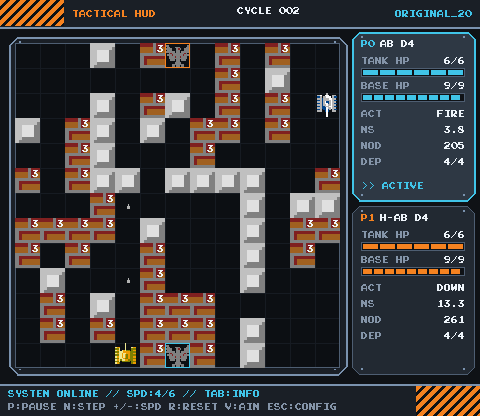
\includegraphics[width=0.93\columnwidth]{figures/ui_battle.png}
\caption{Hai AI trên ORIGINAL\_20. Đây là ảnh minh họa giao diện,
không phải một trong năm kịch bản benchmark.}
\label{t2:fig:ui}
\end{figure}

\code{BulletPlayback} trong \code{presentation.py} nội suy đạn và
hiệu ứng trên dữ liệu hiển thị; không đổi luật ba ô/cycle, HP, va
chạm hoặc quyết định AI. UI đợi hoạt ảnh của lượt trước rồi tiếp tục.
Hệ thống có 40 map: năm tình huống cơ sở và 35 map chuyển từ gốc.
Các map gốc được thích nghi từ 26$\times$26 sang 13$\times$13; nước
thành thép, cỏ/băng thành trống. Bản chạy dùng map đã chuyển trong
\code{levels\_ai/}, không khẳng định giữ mọi cơ chế game gốc.

Bảng Tab hiển thị giá trị, cận, nút, cắt tỉa và chuỗi nước dự đoán
(principal variation, PV). Dấu ``='' là giá trị chính xác; ``$\leq$''
là cận trên của nhánh Alpha-Beta. Không dùng cận như điểm chính xác
để kết luận hai nước bằng nhau. PV chỉ là dự đoán trong cây; agent
lập kế hoạch lại khi tới lượt (Hình~\ref{t2:fig:analysis}).

\begin{figure}[t]
\centering
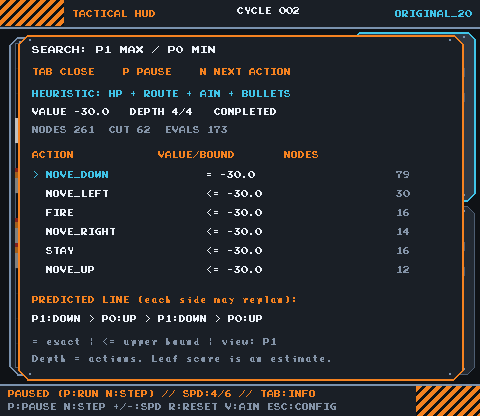
\includegraphics[width=0.93\columnwidth]{figures/ui_search.png}
\caption{Phân tích một quyết định bằng Tab: độ sâu, giá trị/cận và
chi phí tìm kiếm. Ảnh không phải bảng tổng hợp thực nghiệm.}
\label{t2:fig:analysis}
\end{figure}

\subsubsection{Nhập và tích hợp agent nhóm khác}
Đặt file Python trong \code{task2/} hoặc \code{agents/}, nhấn F5 để
làm mới danh sách rồi chọn mục FILE. Loader dùng \code{importlib}, hỗ
trợ factory \code{create\_agent(player\_id)} trả đối tượng có
\code{choose\_action}/\code{act}, hoặc hàm cấp module. Ví dụ giao thức:
\begin{lstlisting}[language=Python]
from game import Action

class MyAgent:
    def __init__(self, player_id):
        self.player_id = player_id

    def choose_action(self, state,
                      time_limit_ms=None,
                      history=None):
        # Replace with the group's search.
        return Action.STAY

def create_agent(player_id):
    return MyAgent(player_id)
\end{lstlisting}
Ví dụ chỉ minh họa tích hợp, không phải cấu hình thứ năm của phép đo.
Loader chuyển \code{time\_limit\_ms}/\code{history} nếu hàm hỗ trợ và
gọi \code{reset} nếu có. Kết quả có thể là Action, tên/số hành động
hoặc tuple (action, info). Hành động được kiểm tra hợp lệ trước khi
áp dụng. Agent ngoài tự tuân thủ deadline mềm; lỗi được ghi nhận,
không biến thành kết quả hợp lệ của thuật toán.

\subsection{Thiết kế thực nghiệm công bằng}
\subsubsection{Nguồn dữ liệu và môi trường}
Số liệu lấy từ \code{experiments/} của dự án \cite{project}, profile
\code{assignment\_four\_modes\_v1}; bản sao CSV và
\code{environment.json} nằm trong thư mục \code{data/} của bộ LaTeX.
Máy đo ghi nhận Linux x86\_64, Python 3.12.14. Chưa có số đo trên
macOS 13.7.8 Intel Core i5 được chỉ định trong đề; không suy diễn
thời gian của môi trường hiện tại thành thời gian máy chấm.

Bộ đo dùng năm kịch bản: \code{default} (11$\times$11, gạch/thép),
\code{open} (9$\times$9 trống), \code{walls} (9$\times$9 có vật cản),
\code{defense} (địch gần căn cứ P0, hướng bắn xuống) và \code{bullet}
(đạn P1 đang tiến về tank P0). Không dùng các ảnh ORIGINAL\_20 để
thay thế kịch bản đo đã công bố.

\subsubsection{Snapshot cùng trạng thái}
Mỗi kịch bản đo cả hai bên, depth 2 và 4, mỗi mode lặp ba lần:
$5\times2\times2\times3\times4=240$ lượt. Mode được xáo thứ tự với
seed 42. Không deadline nên tất cả phải hoàn tất depth yêu cầu.
Các lần lặp cùng snapshot phục vụ đo thời gian, không phải các trận
độc lập. Mỗi phép đo tạo engine/evaluator mới, cache ban đầu rỗng.

Các cặp MM/AB và H-MM/H-AB dùng cùng evaluator, trạng thái, hành động
và depth. Cả bốn mode không TT, tắt \code{track\_pv}; không dựng khóa
PV trong các nút. Sắp xếp con tại gốc áp dụng cho cả hai thuật toán
trong cặp. Thời gian sắp xếp được tính trong tổng thời gian; số lần
đánh giá được tách thành \code{order\_evals} và \code{leaf\_evals},
với tổng bằng \code{total\_evals}. Cache heuristic có thể dùng lại
bên trong một lần tìm kiếm, không dùng chung giữa các phép đo.

Chỉ số gồm ms, số nút vào tìm kiếm (kể cả gốc), lá, số lần cắt, hành
động bị cắt, số lần đánh giá và depth đạt được. Bộ summary có mean/
median theo từng map/bên/depth/mode. Bảng~\ref{t2:tab:search} trong
báo cáo dùng \emph{trung bình trực tiếp trên CSV thô}, 30 lượt cho
mỗi cặp (mode, depth), không lấy trung bình các trung vị.

\subsubsection{Đối đầu đổi bên}
Từ bốn cấu hình có sáu cặp khác nhau; mỗi cặp đấu hai lần đổi P0/P1
trên năm map, tổng $5\times6\times2=60$ trận. Mỗi cấu hình tham gia
30 trận, dùng depth 3, không deadline, PV tắt và agent reset đầu trận.
Cache đường đi được dùng lại trong trận, nên thời gian/nước không
thay thế phép đo snapshot cùng trạng thái.

Bộ chạy dừng sau tối đa 60 cycle. Đây là ngân sách thí nghiệm ngoài
\code{GameState}, không được đưa vào terminal hoặc utility. Nếu chưa
có kết quả, ghi \code{stopped}/\code{unfinished}, không tính hòa.
Phá hủy đúng cycle cuối vẫn ưu tiên kết quả thật. UI không tự kết
thúc ván chỉ vì đạt giới hạn này.

\subsection{Kết quả và phân tích}
\subsubsection{Chi phí tìm kiếm cùng depth}
\begin{table}[t]
\caption{Trung bình 30 lượt cho mỗi mode/depth; thời gian tính bằng ms}
\label{t2:tab:search}
\centering\small
\begin{tabular}{crrrr}
\toprule
Depth / Mode & ms & Nút & Lá & Lần cắt\\
\midrule
2 / MM & 0.357 & 40.6 & 33.8 & 0.0\\
2 / AB & 0.241 & 17.4 & 10.6 & 4.8\\
2 / H-MM & 4.826 & 40.6 & 33.8 & 0.0\\
2 / H-AB & 3.962 & 18.9 & 12.1 & 4.5\\
\midrule
4 / MM & 9.370 & 1329.1 & 1096.1 & 0.0\\
4 / AB & 1.376 & 120.2 & 65.0 & 41.6\\
4 / H-MM & 40.807 & 1329.1 & 1096.1 & 0.0\\
4 / H-AB & 11.579 & 190.7 & 121.7 & 48.2\\
\bottomrule
\end{tabular}
\end{table}

Cả 240 lượt đều hoàn tất depth yêu cầu. Có 60 nhóm (map, bên,
depth, lần lặp), mỗi nhóm kiểm hai cặp cùng evaluator, tổng 120 cặp;
tất cả khớp giá trị tìm kiếm. Hình~\ref{t2:fig:search} trực quan hóa
thời gian và số nút ở depth 4 trên cùng tập snapshot.

\begin{figure*}[t]
\centering
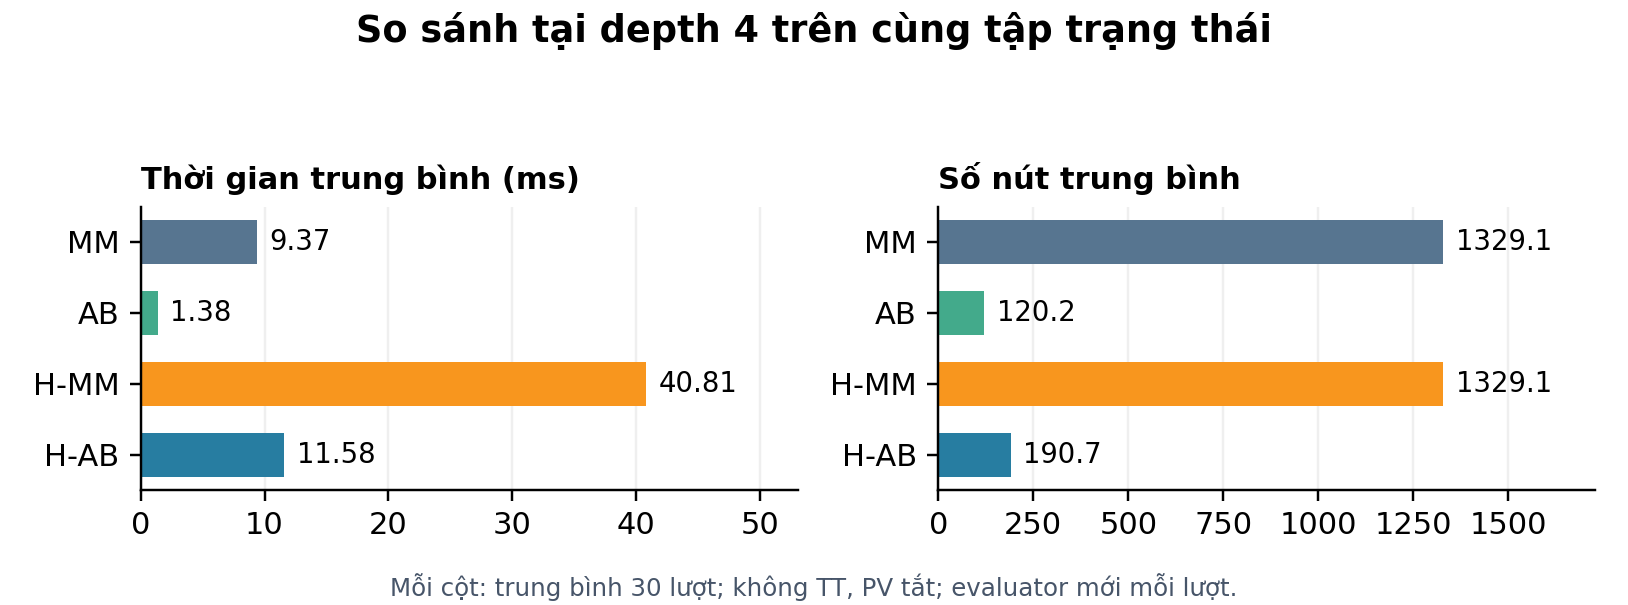
\includegraphics[width=0.95\textwidth]{figures/search_comparison.png}
\caption{Chi phí tại depth 4 trên cùng snapshot và evaluator trong từng cặp.
Mỗi cột là trung bình 30 lượt. Chi phí thấp hơn không tự chứng minh
khả năng chơi tốt hơn.}
\label{t2:fig:search}
\end{figure*}

Đặt $t$ là thời gian trung bình, $N$ là số nút trung bình của cùng
evaluator/depth. Tỷ số thời gian và tỷ lệ giảm nút là
\begin{equation}
S=\frac{t_{\mathrm{MM}}}{t_{\mathrm{AB}}},\qquad
G=1-\frac{N_{\mathrm{AB}}}{N_{\mathrm{MM}}}.
\end{equation}
Ở depth 2, cặp thuần đạt $S=1.48$, $G=57.14\%$; cặp heuristic đạt
$S=1.22$, $G=53.45\%$. Ở depth 4, tương ứng là $6.81$ và $90.96\%$;
$3.52$ và $85.65\%$. Alpha-Beta giảm chi phí trên bộ thử, nhưng mức
giảm phụ thuộc trạng thái và thứ tự duyệt, không phải hệ số cố định.

Heuristic tốn thời gian hơn terminal-only vì tính đường đi, tia ngắm
và dự báo đạn. Điểm trung tính 0 của bản thuần cũng tạo cơ hội cắt
tỉa; ít nút hoặc ít ms hơn không chứng minh bản thuần quyết định tốt
hơn. Cần tách hiệu quả tính toán của cắt tỉa với chất lượng thông tin
đánh giá lá.

\subsubsection{Kết quả đối đầu}
Bảng~\ref{t2:tab:matches} tổng hợp 60 trận. Có 44 trận có bên thắng,
tám hòa do phá hủy đồng thời và tám chưa kết thúc; không có lỗi agent.
Mỗi trận đóng góp hai lượt tham gia vào bảng, nên bốn hàng không phải
120 trận độc lập.

\begin{table}[t]
\caption{Đối đầu depth 3, đổi bên, ngân sách 60 cycle thí nghiệm}
\label{t2:tab:matches}
\centering\small
\begin{tabular}{lrrrrr}
\toprule
Mode & Thắng & Thua & Hòa & Dừng$^{*}$ & ms/nước\\
\midrule
MM & 3 & 19 & 0 & 8 & 3.383\\
AB & 3 & 19 & 0 & 8 & 1.073\\
H-MM & 19 & 3 & 8 & 0 & 12.666\\
H-AB & 19 & 3 & 8 & 0 & 4.940\\
\bottomrule
\end{tabular}
\par\vspace{2pt}\footnotesize
$^{*}$Hết ngân sách khi chưa terminal, không tính hòa; mỗi mode 30 trận.
\end{table}

Hai bản heuristic đều thắng 19/30 trận tham gia, hai bản thuần thắng
3/30 trên bộ thiết lập này. Kết quả phù hợp việc heuristic cung cấp
tín hiệu trước terminal. Tuy nhiên, tỷ lệ gộp gồm nhiều đối thủ và
map cố định, không chứng minh heuristic luôn thắng hoặc suy ra tỷ lệ
thắng trên mọi map. Alpha-Beta giữ chất lượng minimax cùng evaluator/
depth; lợi ích chính ở đây là cắt bớt tìm kiếm.

\subsection{Kiểm chứng tính đúng và giới hạn}
\subsubsection{Kiểm thử}
Bộ kiểm thử lõi gồm 22 trường hợp đã chạy đạt trên môi trường kiểm
tra. Oracle vét cạn độc lập đối chiếu giá trị và hành động tối ưu trên
40 map, cả hai bên, hai evaluator, depth 3. Kiểm tra thêm cận của
Alpha-Beta, tính hợp lệ của PV và việc tìm kiếm không sửa trạng thái
gốc. Cây tính tay $\max(\min(3,5),\min(2,9))=3$ xác nhận hai thuật
toán cùng giá trị và Alpha-Beta bỏ được một lá.

Kiểm thử luật bao gồm đi một ô, quay khi bị chặn, đạn ba bước với va
chạm từng ô, HP gạch/tank/base, đạn gặp nhau, tank bước vào đạn và sát
thương phe mình. Các trường hợp terminal xác nhận phá hủy đồng thời,
cycle lớn không tự hòa, cap ngoài game ghi unfinished và phá hủy
ở cycle cuối vẫn tính kết quả thật. Tắt PV không đổi điểm/nước;
benchmark tạo engine/evaluator mới và tổng đánh giá bằng đánh giá
gốc cộng đánh giá lá. Kiểm tra bổ sung xác nhận UI, map chuyển,
nạp AI ngoài và phần phát lại không đổi trạng thái.

\subsubsection{Giới hạn và hướng cải thiện}
Tìm kiếm hữu hạn không bảo đảm tối ưu cả ván. Baseline terminal-only
thiếu tín hiệu ở độ sâu nhỏ nên có thể lặp FIRE; cần xem điểm/depth
thực và kiểm thử oracle thay vì chỉ suy luận qua chuyển động tank.
Mô hình đường đi/dự báo đạn là gần đúng và trọng số chưa được kiểm
định độ nhạy. Bộ đo hiện có năm kịch bản cố định, chưa có kết quả
đối đầu cùng ngân sách thời gian hoặc đo trên máy macOS của đề.

Hướng phát triển là mở rộng snapshot chiến thuật hợp lệ, đo depth
thực dưới cùng deadline, tiếp tục đổi bên và thử agent nhóm khác.
Những phép đo này cần ghi riêng cấu hình; không thay số liệu đã công
bố hoặc thêm luật hòa nhằm làm các baseline kết thúc sớm.

\subsection{Kết luận và cách tái hiện}
Hệ thống đáp ứng các thành phần mô hình trò chơi zero-sum, bốn cấu
hình đối kháng, tổ chức hướng đối tượng, UI Pygame và giao thức nhập
AI. Luật HP, di chuyển, đạn từng ô và terminal được dùng chung cho
search và game. Trong phạm vi đã đo, Alpha-Beta giữ giá trị Minimax
và giảm chi phí; heuristic cải thiện kết quả đối đầu với chi phí đánh
giá lớn hơn. Phạm vi kết luận được giới hạn bởi map, depth, ngân sách
và môi trường thực nghiệm đã công bố.

Chạy từ thư mục mã nguồn chứa \code{tanks.py}:
\begin{lstlisting}[language=bash]
python -m pip install -r requirements.txt
python tanks.py
python -m unittest discover -s tests -v
\end{lstlisting}
Phụ thuộc game là \code{pygame>=2.5,<3}. Các lệnh sau tái hiện thí
nghiệm và ghi CSV mới ở thư mục hiện tại, không ghi đè bộ tham khảo:
\begin{lstlisting}[language=bash]
python task2/benchmark.py --scenarios default open walls defense bullet --players both --depths 2 4 --repeats 3 --output benchmark_results.csv --summary benchmark_summary.csv
python task2/tournament.py --scenarios default open walls defense bullet --depth 3 --max-cycles 60 --output tournament_results.csv --summary tournament_summary.csv
\end{lstlisting}
Bốn CSV tham khảo gồm dữ liệu thô và bảng tổng hợp của benchmark
snapshot và đối đầu, lưu trong \code{experiments/} của mã nguồn và
được sao chép vào \code{data/} của bộ báo cáo. Thời gian chạy lại có
thể khác theo máy/tải hệ thống; các bảng ở đây dùng nguyên số đo đã
lưu, không giả định mọi lần chạy cho cùng ms.

% File nội dung Bài toán 3. Không thêm documentclass/begin{document}.
% Thay tên và bổ sung nội dung theo đề thực tế; chưa có thông tin để viết thay.
\section{Bài toán 3: Tên bài toán cần bổ sung}
\label{sec:task3}
\textit{Phần nội dung Bài toán 3 do thành viên phụ trách bổ sung.}
% \subsection{Phát biểu và mô hình hóa bài toán}
% \subsection{Thuật toán và cài đặt}
% \subsection{Thực nghiệm và phân tích kết quả}
% \subsection{Kết luận và hạn chế}


\balance
\begin{thebibliography}{00}
\bibitem{assignment}
Đề bài học phần Introduction to AI, ``Task 2: Adversarial Search ---
Tank Battle Game,'' tài liệu đề bài được cung cấp cho dự án.
\bibitem{battlecity}
Raitis G., ``Battle City Tanks,'' mã nguồn và tài nguyên game.
[Trực tuyến]. \url{https://github.com/raitisg/battle-city-tanks}.
\bibitem{pygame}
Pygame, ``Pygame documentation.''
[Trực tuyến]. \url{https://www.pygame.org/docs/}.
\bibitem{project}
Nhóm thực hiện, ``NMTTNT: Tank Battle,'' mã nguồn, kiểm thử và dữ liệu
thực nghiệm. [Trực tuyến]. \url{https://github.com/baam2603/NMTTNT}.
\end{thebibliography}
\end{document}
